\section{PCStream}
In this section, we describe in detail our proposed automatic stream management technique.
First, we explain how to obtain a PC, which is a lifetime hint of application data, at the system level. 
We then describe the overall architecture of PCStream with how to allocate stream using the PC information. 
Finally, we introduce an exceptional case with an optimization technique for the case.

\subsection{Getting the program context}
As mentioned earlier, we define the PC as the addition of instruction counter values along the 
execution path of the function call reaching the write. 
(In general, the function call process involves pushing the current instruction 
counter to the return address of the process stack.) 
Back tracing the stack and collect the return address can easily be done using the frame pointer register. 
However, when using the {\tt -fomit-frame-pointer} compile option of GCC, 
the general back tracing is impossible because frame pointer register is used for the general purpose~\cite{GCC}. 
Instead, we search from the top to bottom of the stack and regard the stack value 
belonging to the code area of the process as the return address. 

\begin{figure}[t]
	\centering
	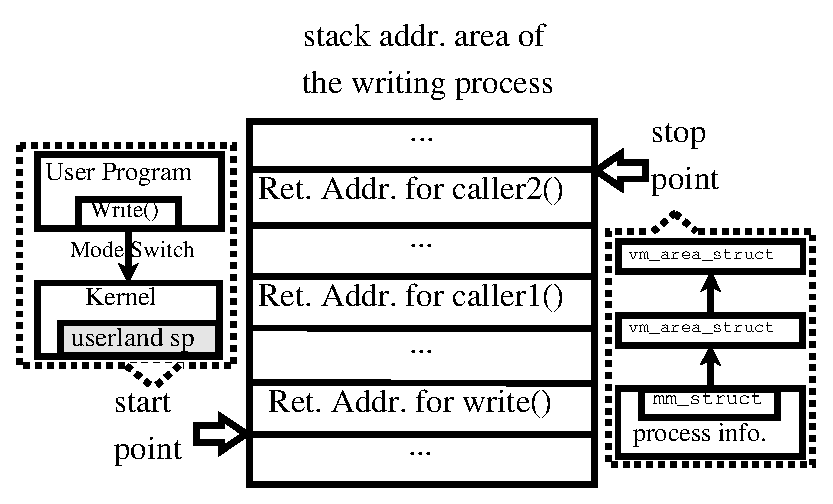
\includegraphics[width=0.7\linewidth]{figure/getpc}
	\caption{PC calculation method}
	\label{fig:getpc}
	\vspace{-20pt}
\end{figure}


Figure~\ref{fig:getpc} shows the procedure. 
The start address of the user process stack search is the stack pointer value of user space ({\it userland sp})
that is maintained for returning from the kernel mode. 
The end address of the search is the last address of the virtual memory unit space ({\tt vm\_area\_struct}) 
containing userland sp from the process's virtual memory information ({\tt mm\_struct}). 
The scope of the code area of the process is easily obtained from the virtual memory information. 
In order to reduce the search time, we finish the searching 
when we find return addresses more than the threshold.
(Experimental results for various programs showed that different execution paths could be distinguished 
from each other only by a threshold value of 5 or less.)
The sum of all the address values found during the searching is used 
as the representative PC value of the context.
This process takes 300 to 400 nanoseconds on a 3.4 GHz CPU machine, 
so we can say the overhead is not huge.
Moreover, since we can calculate PC once per write system call,
the overhead is further decreased for long-length writes.


\subsection{Overall Architecture of PCStream}
Figure~\ref{fig:architecture} shows the overall architecture of PCStream.
When a write request occurs, the PC value is calculated by searching the stack area of the writing process.
In the example of Figure~\ref{fig:architecture}, data {\tt D0} and {\tt D1} with 
different execution paths are recognized as PC IDs 0 and 1, respectively.
PCStream analyzes the lifetime of each PC and maps the appropriate one of the available streams.
In this paper, since we focus on to show the feasibility of the PC-based approach, 
the number of application programs is limited to one, 
and PC and stream are mapped to 1: 1.

\begin{figure}[t]
	\centering
	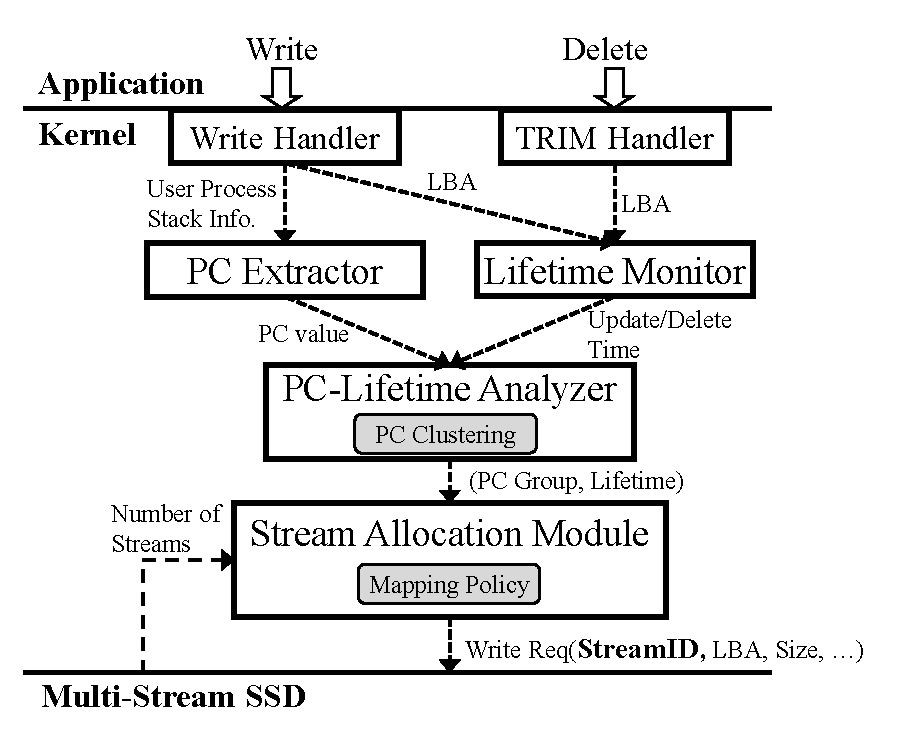
\includegraphics[width=0.5\linewidth]{figure/architecture}
	\caption{The overall architecture of PCStream}
	\label{fig:architecture}
	\vspace{-20pt}
\end{figure}


In the example shown in the Figure~\ref{fig:architecture}, PC0 is assigned 
to stream 0 and PC1 is assigned to stream 1.
The function of dynamically adjusting the mapping between PC and stream 
according to the change of operation environment is left as a future work.
For example, the number of PCs can be larger than the number of available streams
due to the multiple applications or a large number of PCs of an application.
For the case, the lifetime analyzer and PC clustering technique are required so that 
the lifetime of each PC data is analyzed to allocate PCs having a similar lifetime to the same stream.
Also, dynamic m: n mappings are needed to dynamically respond to changes in 
application's write pattern or number of supported streams.

The stream number determined according to the PC value is maintained in the inode of the file, 
and is transmitted as the stream number when the write request is issued to the device. 
The data of the transmitted request is stored in the physically separated area 
in the SSD according to the specified stream number.


\subsection{PCs of various lifetimes and substreams}
According to our observations, the lifetime of data is similar 
for contexts with simple operations such as log, as shown in section 2, 
but some contexts generate various lifetime data.
The compaction behavior of RocksDB belongs to a such context.
Compaction moves the flushed data to the different levels
of the LSM-tree~\cite{RocksDB}, 
so the data generated in one compaction context has 
different life characteristics depending on the target level.
Like RocksDB, LSM-tree-based DBs tend to have a longer 
data lifetime at lower levels~\cite{Level}.
Since the allocated capacity increases as the level goes down, 
the cycle of compaction, which deletes files, is long at low level.
In order to see the difference in the lifetime of each compaction target level,
we modified the RocksDB code to distinguish files according to the compaction level.
Figure~\ref{fig:compaction} shows the lifetime distribution of 
different compaction level data and compaction context data.

\begin{figure}[!t]
\centering
\hspace{1pt}
\subfloat[compaction:L2]{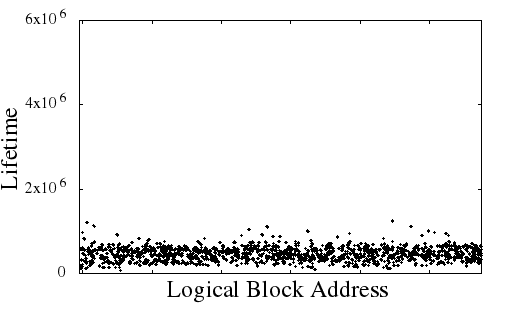
\includegraphics[width=0.23\textwidth]{figure/type_4}}
\subfloat[compaction:L3]{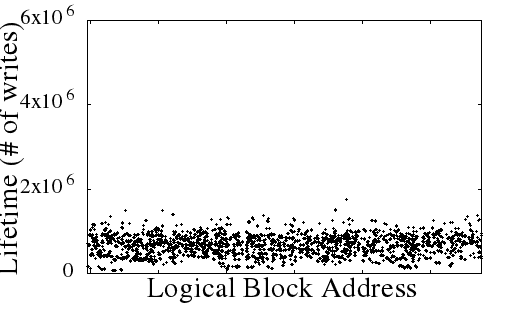
\includegraphics[width=0.23\textwidth]{figure/type_5}}
\hfill
\vspace{-10pt}
\subfloat[compaction:L4] {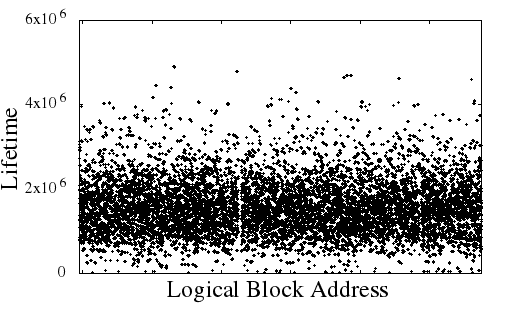
\includegraphics[width=0.23\textwidth]{figure/type_6}}
\subfloat[PC ID: \#4]{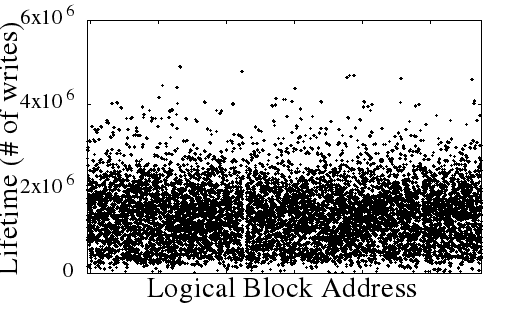
\includegraphics[width=0.23\textwidth]{figure/pc_3}}
\vspace{-10pt}
\caption{The lifetime distribution of compaction context.} 
\label{fig:compaction}
\vspace{-25pt}
\end{figure}

Level 2 data in Figure~\ref{fig:compaction}(a) and 
level 3 data in Figure~\ref{fig:compaction}(b) seem to have 
a limited lifetime due to the frequent compaction.
On the other hand, because of the long compaction period 
due to the largest space of LSM-tree's lowest level, 
the lifetime is longer than other levels as shown in ~\ref{fig:compaction}(c).
Also, since the target file of the compaction is determined 
by the range of key values of the file~\cite{RocksDB}, 
the previously created file can be deleted 
by participating in the compaction. 
Therefore, the data stored at the lowest level has a very wide lifetime.
However, since all of these data are created in the same context, 
PC 4 can not distinguish any data of the compaction as shown in ~\ref{fig:compaction}(d).
In order to overcome the limitation of PC-based data classification,
we suggest a new optimization technique for multi-stream SSD 
rather than asking application to differentiate the compaction function according to its level.

Basically, the reason for distinguishing data of a similar lifetime is 
to match the timing of data invalidation. 
If long-lived data is gathered together excluding short-lived data, 
there would be no significant impact on WAF. 
So if we store the long-lived data separately even after 
the data is written to the wrong stream, 
we can greatly reduce the side effects of the limitation. 
Therefore, we consider a valid page copied during the GC 
as a misplaced long-lived data 
and allocate a separate substream to accommodate it. 
For example, if a PC with various lifetimes is assigned to stream A, 
we define stream A' as a substream of A and 
move the valid page of stream A to stream A' during GC. 
This prevents long lifetime data of stream A from being repeatedly copied 
by GC.



